\chapter{Measurement Results}
\label{ch:MeasureRes}

\author{Nico Leidenfrost}
%
In order to test GRAMOC, a test scenario had to be created. As an abstraction to the magnetometer, an accelerometer was used. The mathematical model to process the accelerometer sensor data is the same as the one form the magnetometer data which is ultimately used. The reason that a alternative had to be used is that the development of the gradient magnetometer was delayed during the writing of this thesis. Also acceleration is easier to influence without using scientific items.

To get example sensor readouts from the accelerometer, the sensor was mounted inside a car.

\section{Car Mount}

To mount the GRAMOC setup in a car, the 12V DC on-board power supply had to be inverted to 230V AC. This was necessary to power an access point as GRAMOC works over an internet connection. The two Raspberry Pis were powered by a powerbank. The Raspberry Pi that acted as sensor was taped to the arm rest of the car. This setup is depicted in figure \vref{fig:CarMount}.

\begin{figure}[h]
    \centering
    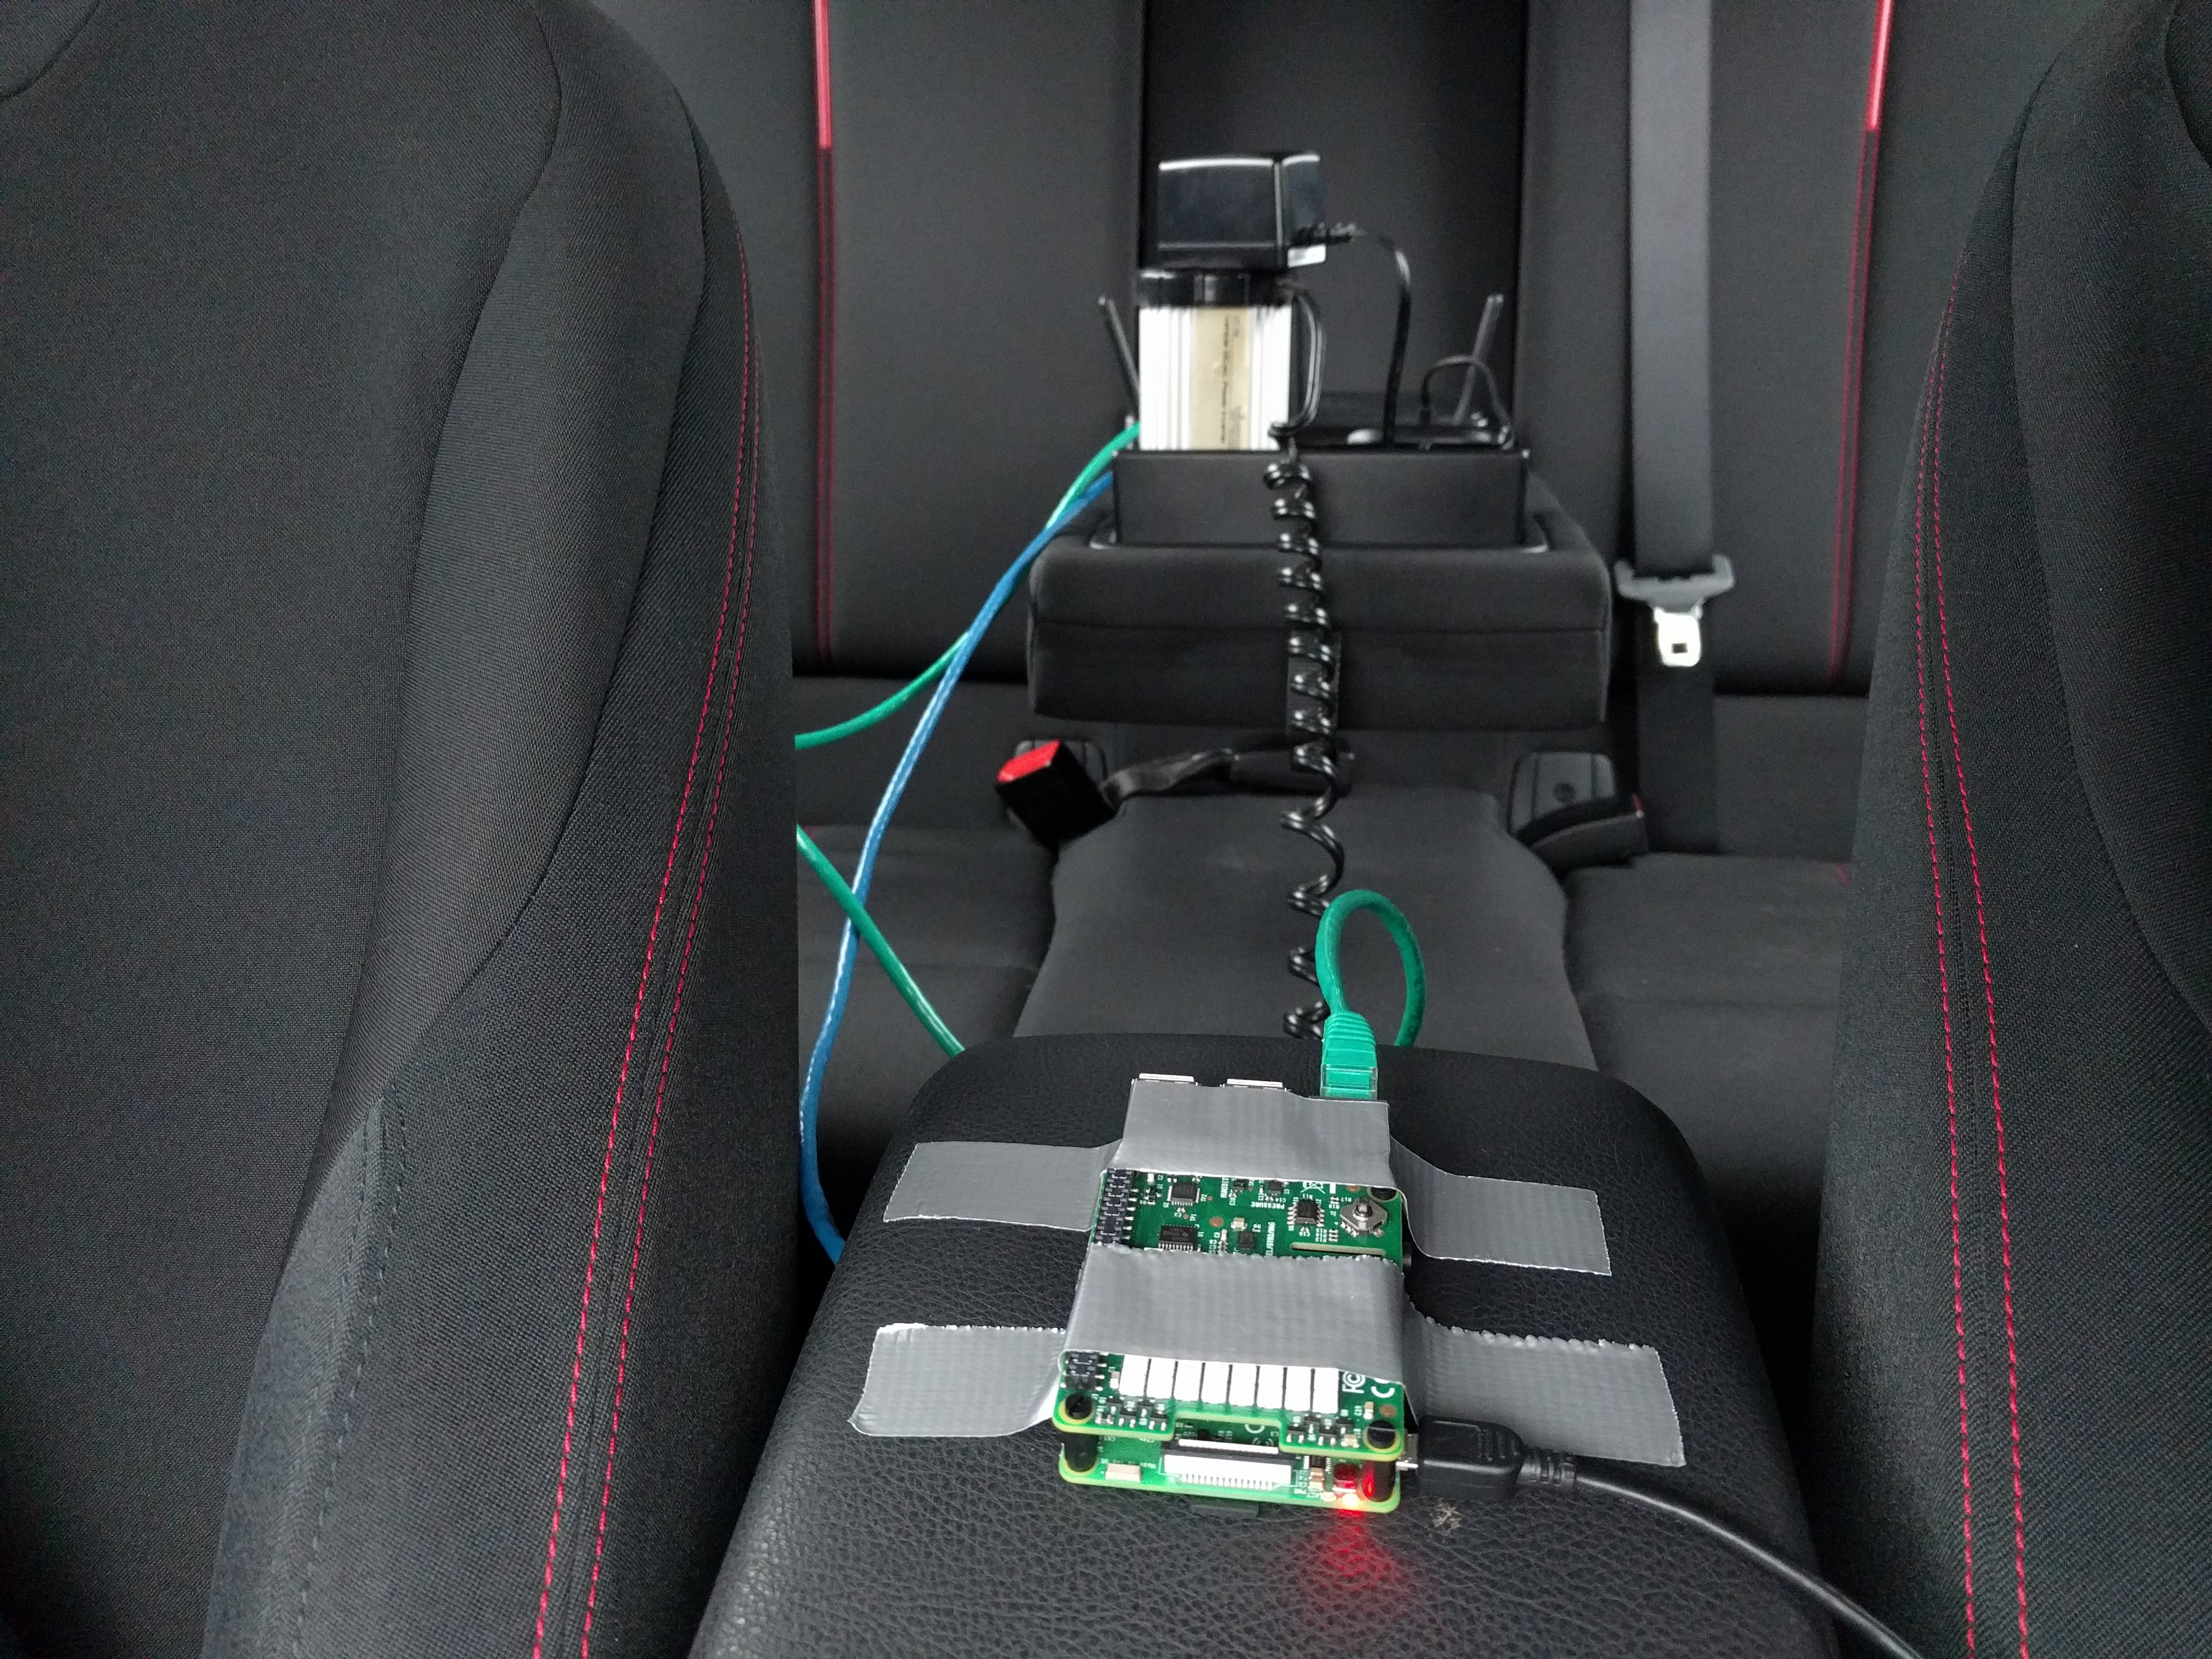
\includegraphics[width=10cm,keepaspectratio]{car_mount}
    \caption{Car Mount of the Raspberry Pi accelerometer}
    \label{fig:CarMount}
\end{figure}

\section{Test Scenarios}
To demonstrate the real-time plotting capabilities, a few scenarios were chosen in which it is easy to understand the recorded data. These scenarios are:

\begin{itemize}
    \item Shifting gears
    \item Driving in a roundabout
    \item Emergency braking
    \item Oversteering
\end{itemize}

As the used sensor is an accelerometer, the measured sensor data represent g-forces. The x axis represents the forward acceleration of the car, the y axis represents the lateral acceleration and the z axis represents the vertical acceleration. In the way the sensor was positioned, positive values on the x axis represent forward acceleration and negative values represent backward acceleration. Since the y axis displays the lateral acceleration, positive values represent a right turn and negative values represent left turns.

\subsection{Shifting Gears}
The first demonstration scenario is shifting gears while driving. Every time a driver shifts to another gear, the acceleration is interrupted. This short interruption is documented by the red line, which represents the forward acceleration, in figure \vref{fig:ShiftGears}. It can be observed that every time the driver shifts to another gear the line drops back to zero. The example in figure \vref{fig:ShiftGears} shows that the driver shifts 3 times from  first to fourth gear.

\begin{figure}[H]
    \centering
    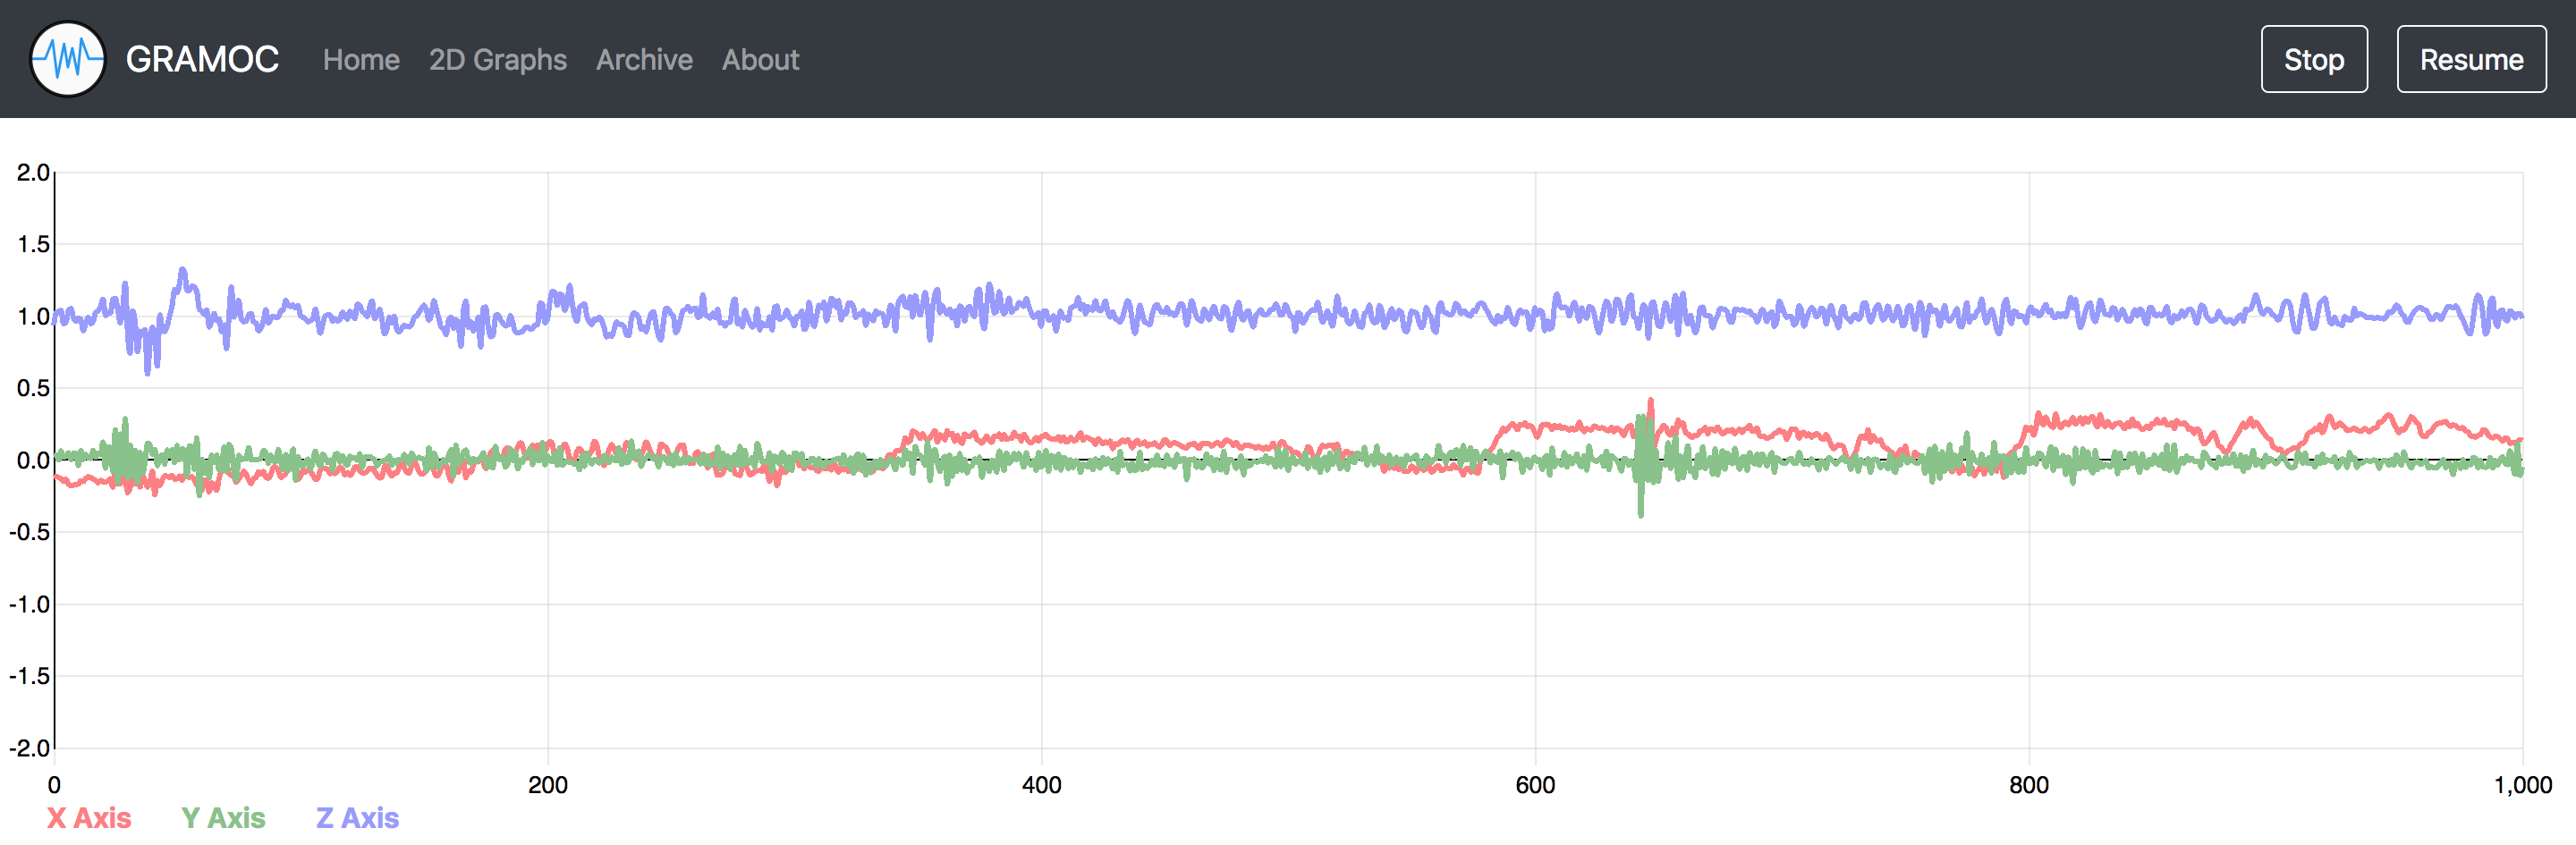
\includegraphics[width=15cm,keepaspectratio]{shift}
    \caption{Measured sensor data when shifting gears}
    \label{fig:ShiftGears}
\end{figure}

\subsection{Driving in a Roundabout}
In the second scenario, a driver is driving through a roundabout. This scenario was chosen to be used as an example, because it is a situation where the lateral acceleration is roughly the same all the time. As shown in figure \vref{fig:Roundabout}, the forward acceleration stays around zero the whole time and the lateral acceleration is located about -0.5g. The reason why the acceleration remains stable the whole time is simply because when driving through a roundabout, a driver should drive with constant speed and turn.

\begin{figure}[H]
    \centering
    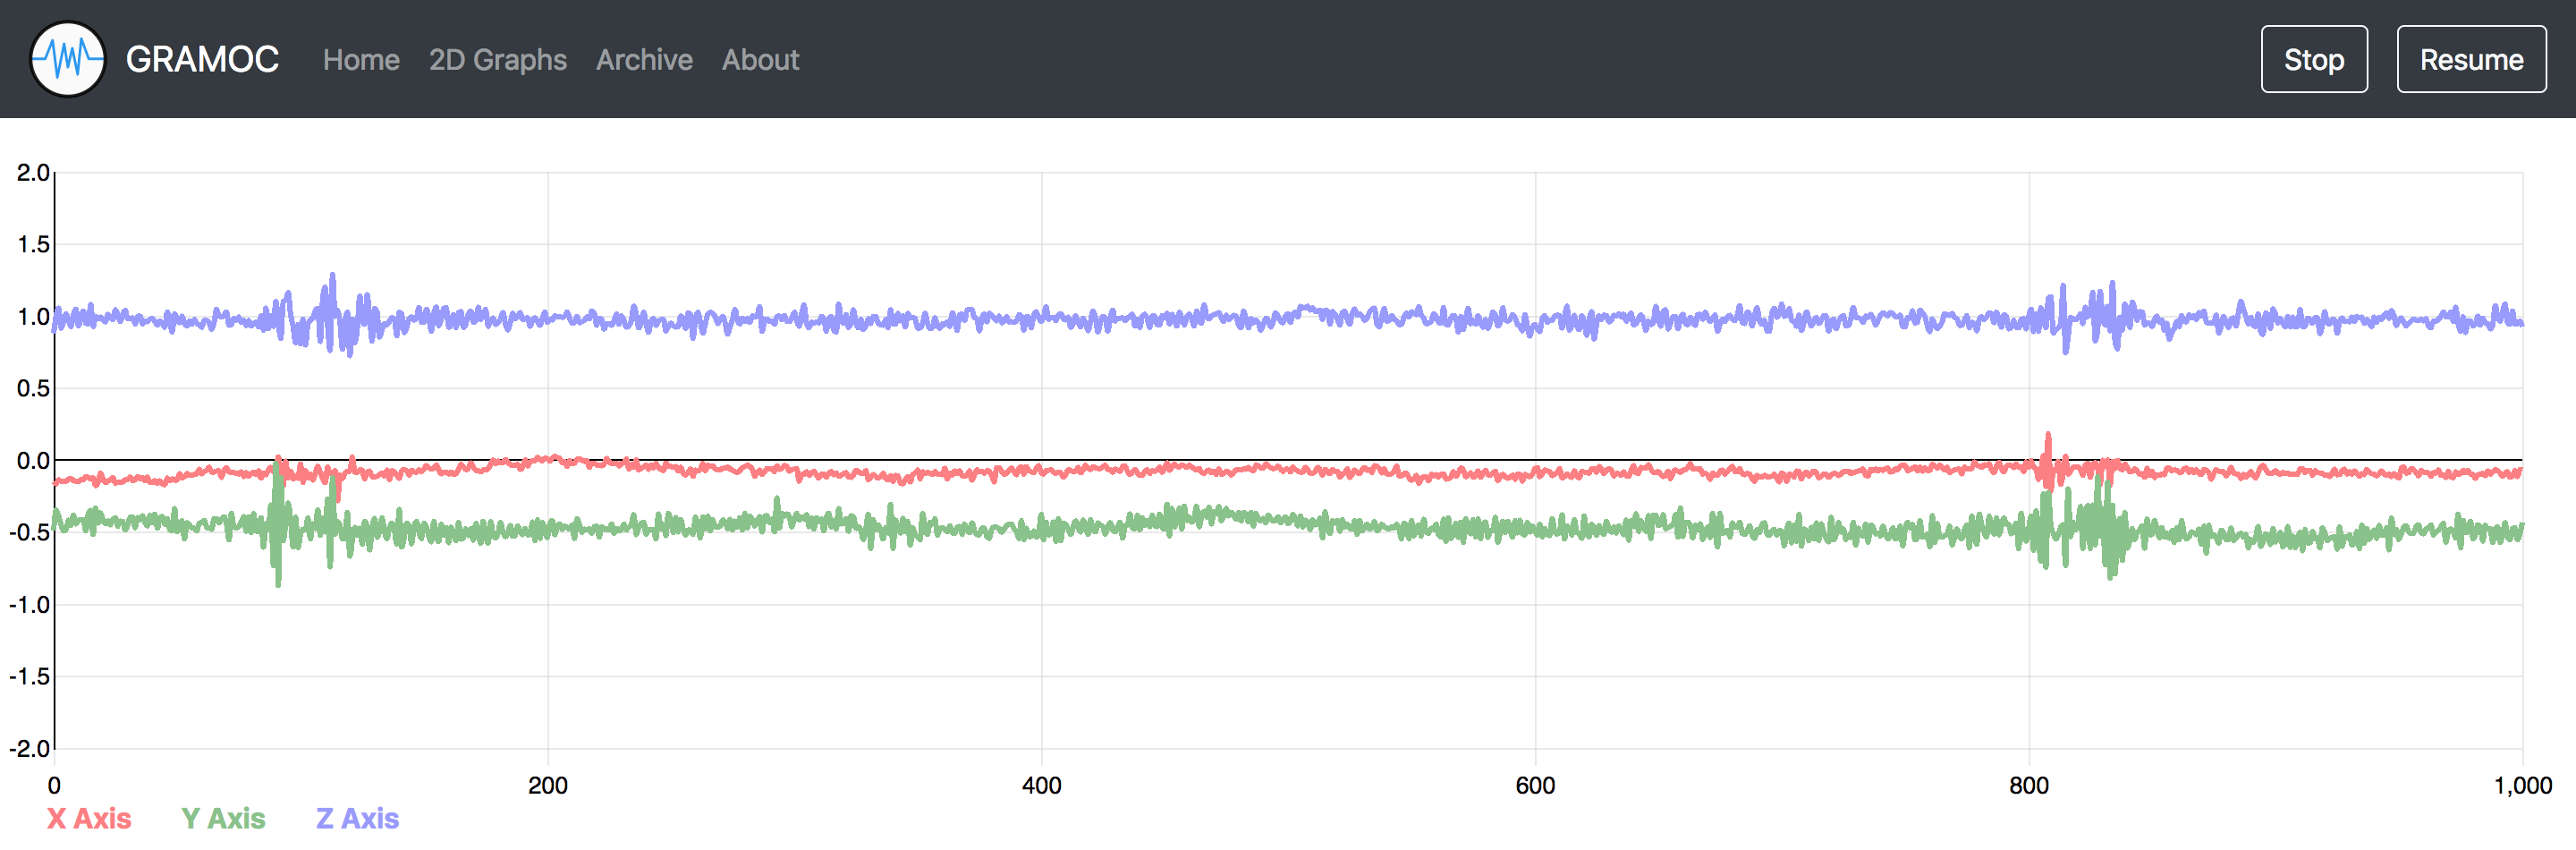
\includegraphics[width=15cm,keepaspectratio]{roundabout}
    \caption{Measured sensor data when driving in a roundabout}
    \label{fig:Roundabout}
\end{figure}

\subsection{Emergency Breaking}
Another scenario where acceleration can be easily shown is the case of emergency braking. When a driver needs to stop his car immediately because there are for example people in front of the car, there needs to be a massive amount of negative acceleration, depending on the current velocity of the car. The acceleration force of such a maneuver is depicted in figure \vref{fig:EmBrake}. The example below shows a driver who is driving at a steady speed of 30 km/h at first and then stops the car immediately. While braking the measured g-force reached a maximum of -1.1g.

\begin{figure}[H]
    \centering
    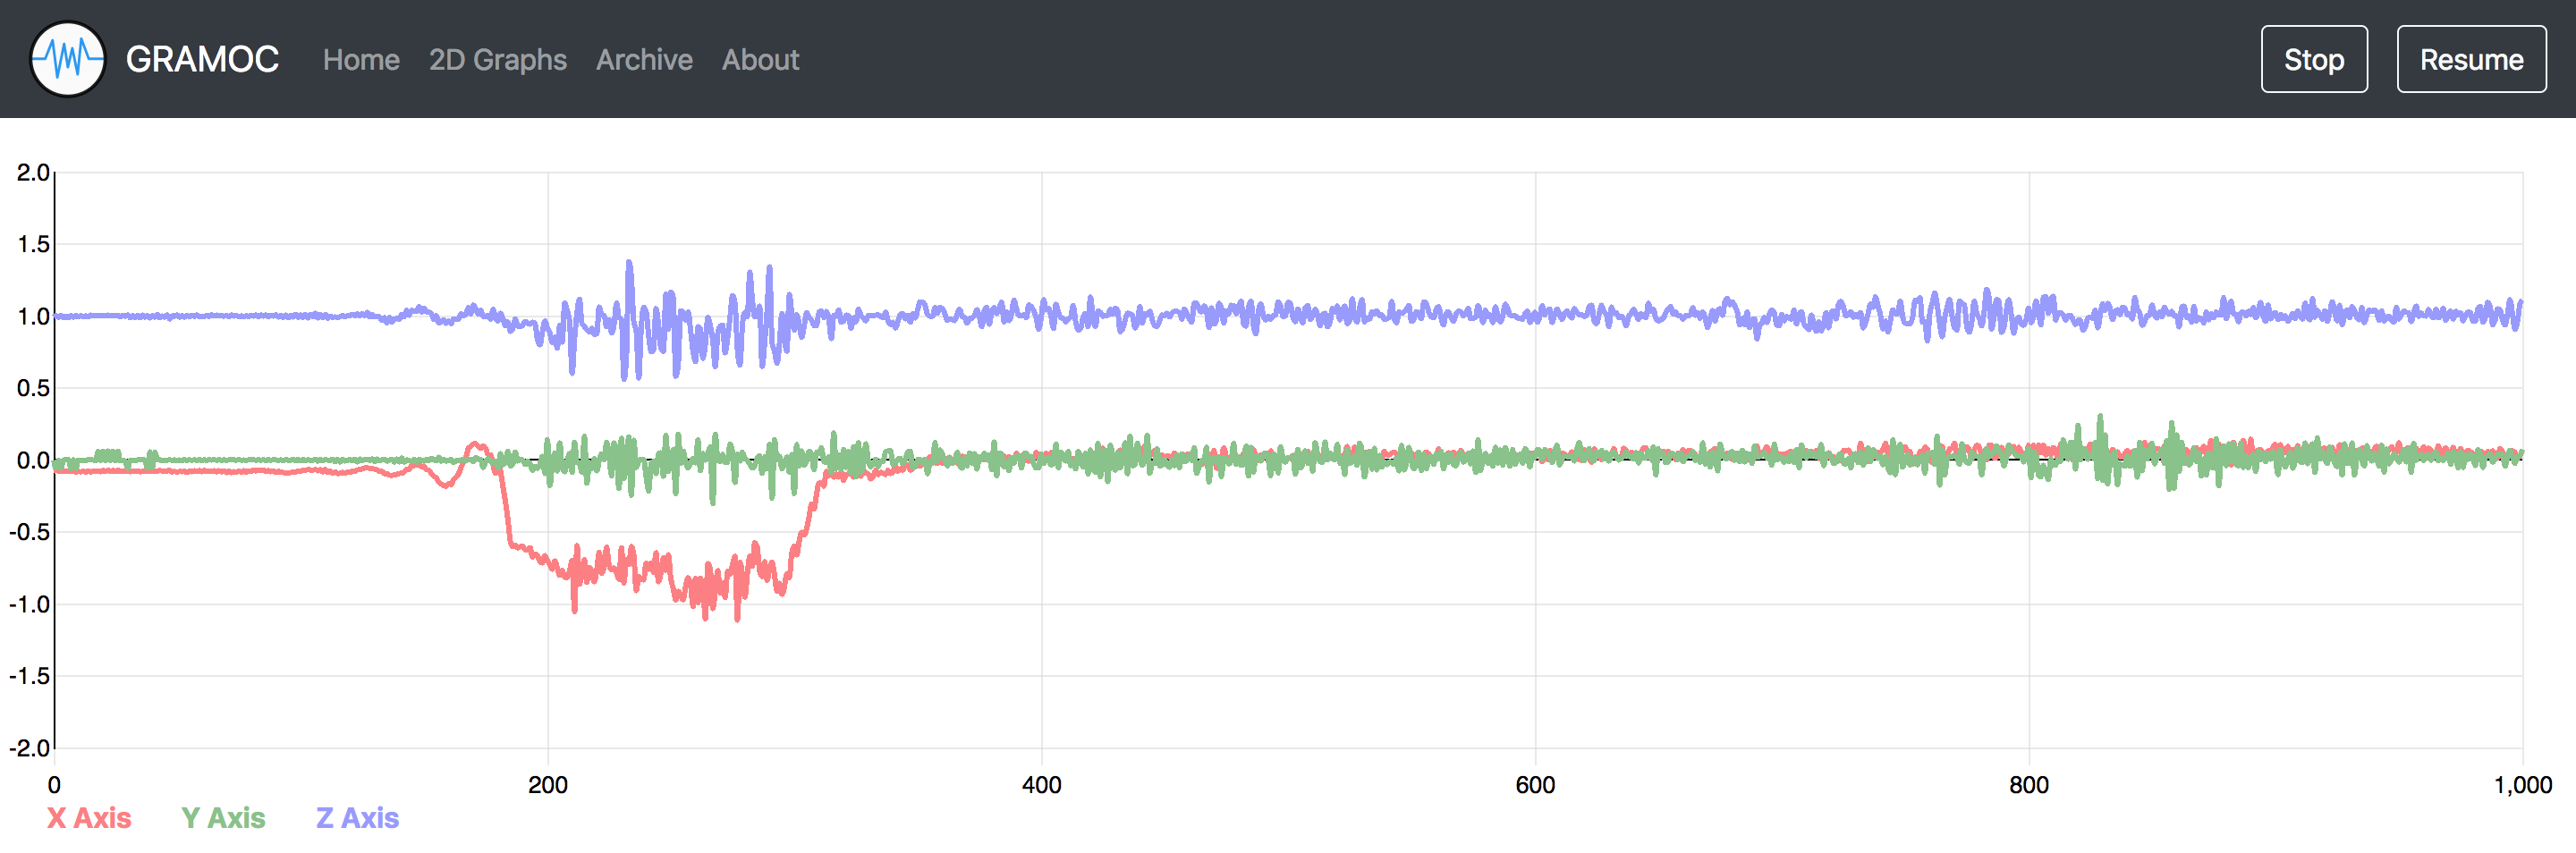
\includegraphics[width=15cm,keepaspectratio]{brake}
    \caption{Measured sensor data when applying an emergency brake}
    \label{fig:EmBrake}
\end{figure}

\subsection{Oversteering}

The last scenario was chosen to show how a car behaves when it is temporarily out of control. This could happend during oversteer caused by a wet street. As depicted in figure \vref{fig:Oversteer} the forward acceleration is erratic, but above zero the whole time during the oversteer phase. The green line which represents the lateral acceleration fluctuates between 1.0g and -1.0g for a short duration, in the remaining time the line stays below zero, due to the fact that the maneuver was applied in a left turn.

\begin{figure}[H]
    \centering
    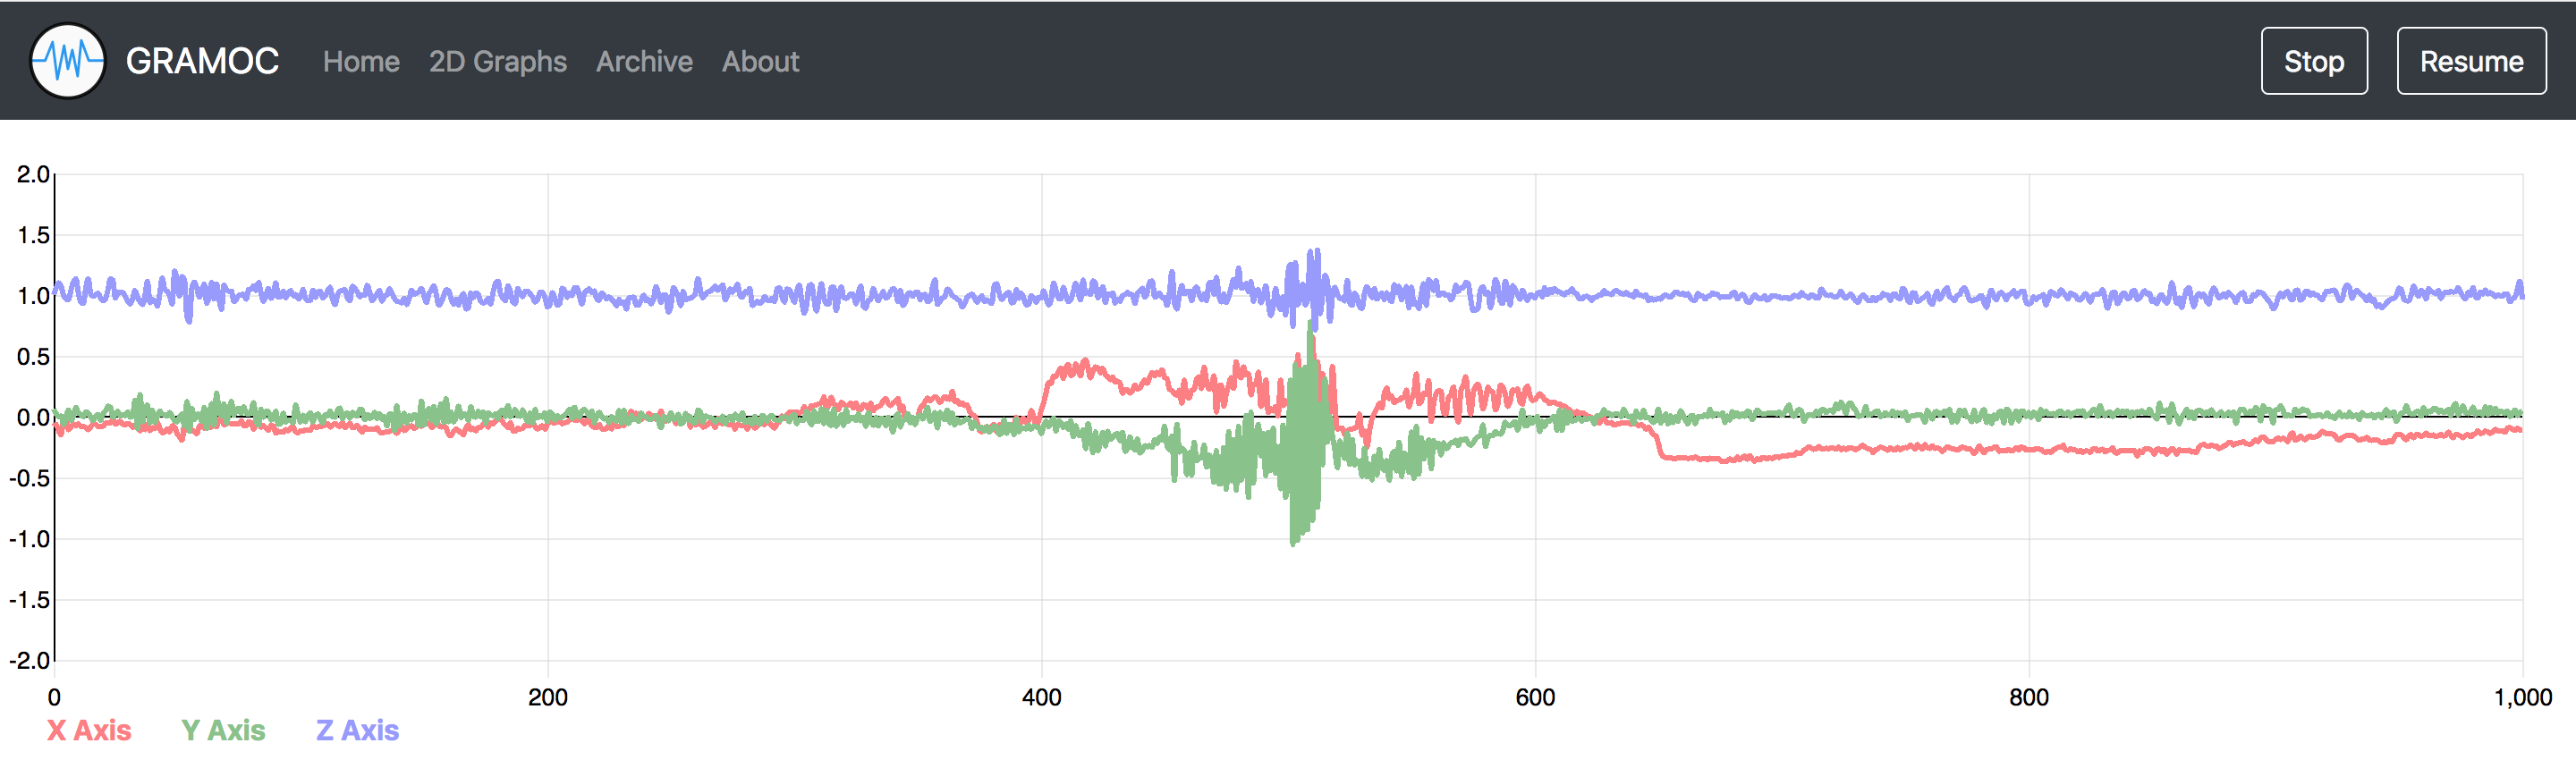
\includegraphics[width=15cm,keepaspectratio]{drift}
    \caption{Measured sensor data when oversteering}
    \label{fig:Oversteer}
\end{figure}

\section{Regression Results}

% was genau wurde gemacht?
% wie verhaelt sich der test zu den stahlbaendern?
% wie wurde untersucht (zwei fahrer, einer langsam einer schnell)
% was wurde berechnet?
% variablen, x y Beschl, timestamp (warum z Beschl unwichtig?)

% Ergebnisse
% warum funktionierts auf 'normaler' strecke nicht so gut? (gleichbleibende geschw => 0 beschl (sind ja brave fahrer die sich an die stvo halten ;-)))
% wie gut funktionierts im kreisverkehr (mittelwert? stdev? ausreisser?)

To test the multiple linear regression capabilities of GRAMOC, another test scenario had to be created. During these tests, it was tried to predict the driver of the car using the acceleration data from the sensor. It was decided to only use forward and lateral acceleration, as the vertical acceleration mostly depends on parameters like road condition. To link the acceleration data to the driven route a timestamp was taken as the third variable.

\subsection{Course 1}

The first test used a predefined route that is depicted in figure \vref{fig:ziss_route}. This route was driven by two sample drivers. One that drives rather quick and one slow driver. These drivers were numerically represented by 1 and 2.

\begin{figure}[H]
    \centering
    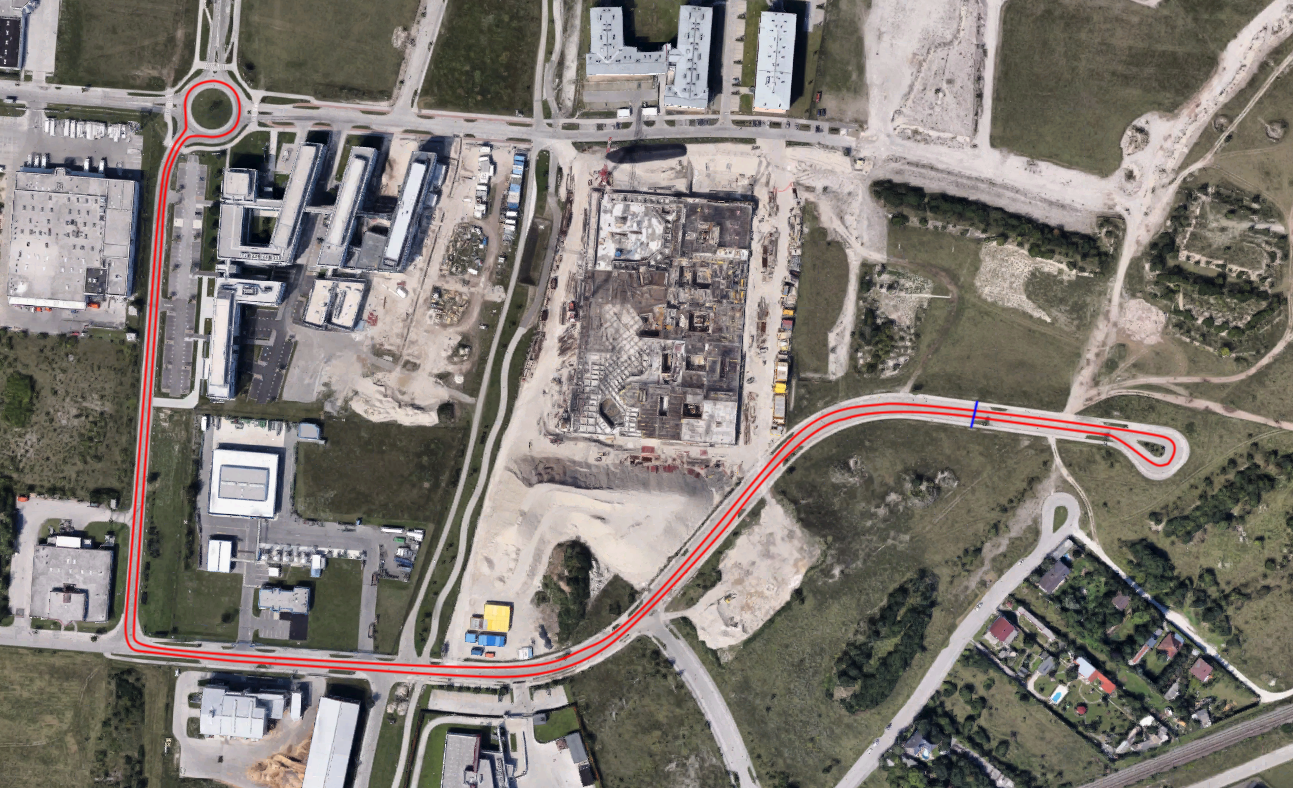
\includegraphics[width=\textwidth,keepaspectratio]{ziss_route}
    \caption{Satellite view of the test route. Image taken from Google Maps}
    \label{fig:ziss_route}
\end{figure}

After completing the two runs, GRAMOC tried to predict the driver. As GRAMOC uses streaming data, the prediction can not simply be shown at the end of the program, as this would be too inaccurate. Therefore only the average prediction is shown after the program finishes. The prediction data itself is still getting calculated in real-time. Also the minimum, maximum and standard deviation of the average are calculated. The obtained results after testing this with the driving style of the two sample drivers are shown in table \vref{tab:prediction1}.

\begin{table}[H]
\centering
\begin{tabular}{|l|l|}
\hline
\textbf{Driving Style} & \textbf{Prediction} \\ \hline
1                      & 1.4                 \\ \hline
2                      & 1.8                 \\ \hline
\end{tabular}
\caption{Prediction from the first regression testing phase}
\label{tab:prediction1}
\end{table}

These predictions only allow to identify tendencies, but do not predict the driver precise enough.

After researching thoroughly, it was decided to use a course that does not have long straights as these were identified to mislead the regression model. This happens because on long straights the car mostly reaches the speed limit of the road and then does not have any acceleration. And no acceleration can not be matched with a driver.

\subsection{Course 2}

The second course had to be windy. The easiest way to get a lot of acceleration is to drive through a roundabout. In a roundabout there will always be at least some acceleration, so this was taken as the second course. For the sake of simplicity the roundabout that was used in the first course (see figure \vref{fig:ziss_route}) was used as this test-roundabout.

The procedure was the same as in the first test, two drivers drive the roundabout at whichever speed they like. After this two runs one driver drives again and GRAMOC tries to predict him. This time, the results were much better as depicted in table \vref{tab:prediction2}.

\begin{table}[H]
\centering
\begin{tabular}{|l|l|l|}
\hline
\textbf{Driving Style} & \textbf{Prediction} & \textbf{Standard Deviation} \\ \hline
1                      & 0.97                & 0.18 \\ \hline
2                      & 1.99                & 0.09 \\ \hline
\end{tabular}
\caption{Prediction from the second regression testing phase}
\label{tab:prediction2}
\end{table}

